% --------------------------------------------------------------------------------

\begin{exercise}[Exercise 3.17]

What is the Bellman equation for action values, that is, for $q_\pi$?
It must give the action value $q_\pi(s, a)$ in terms of the action values, $q_\pi(s_0, a_0)$, of possible successors to the state-action pair $(s, a)$.
Hint:
the backup diagram to the right corresponds to this equation.
Show the sequence of equations analogous to \eqref{eq:2.15}, but for action values.

\begin{figure}[H]
    \centering
    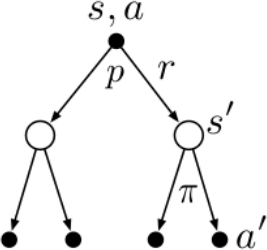
\includegraphics[width = 0.2 \textwidth]{2.17.png}
    \caption{$q_\pi$ backup diagram}
    \label{fig:2.17}
\end{figure}

\end{exercise}

% --------------------------------------------------------------------------------

\begin{solution}

ToDo!

\end{solution}

% --------------------------------------------------------------------------------
